\documentclass[letterpaper,pdftex]{article}

\setlength{\textwidth}{168mm}
\setlength{\textheight}{210mm}
\setlength{\oddsidemargin}{0cm}
\setlength{\topmargin}{0cm}
\setlength{\headheight}{48pt}
\addtolength{\textheight}{-25pt}
\voffset -0.5in

\usepackage{natbib}
\usepackage[utf8]{inputenc}
\usepackage[spanish]{babel}
\usepackage{xcolor,graphicx}
\graphicspath{{Figures/}}
\usepackage{fancyhdr}
\usepackage{multirow}
\usepackage{siunitx}
\usepackage{hyperref}
\hypersetup{
    colorlinks,
    citecolor=blue,
    filecolor=black,
    linkcolor=blue,
    urlcolor=black
}
\usepackage{epstopdf}
%To code editing
\usepackage{listings}
\usepackage{xcolor}
\definecolor{codegreen}{rgb}{0,0.6,0}
\definecolor{codegray}{rgb}{0.5,0.5,0.5}
\definecolor{codepurple}{rgb}{0.58,0,0.82}
\definecolor{backcolour}{rgb}{0.95,0.95,0.92}

\lstdefinestyle{mystyle}{
    backgroundcolor=\color{backcolour},   
    commentstyle=\color{codegreen},
    keywordstyle=\color{magenta},
    numberstyle=\tiny\color{codegray},
    stringstyle=\color{codepurple},
    basicstyle=\ttfamily\footnotesize,
    breakatwhitespace=false,         
    breaklines=true,                 
    captionpos=b,                    
    keepspaces=true,                 
    numbers=left,                    
    numbersep=5pt,                  
    showspaces=false,                
    showstringspaces=false,
    showtabs=false,                  
    tabsize=2
}

\lstset{style=mystyle}

% -------------URL style
\hypersetup{
    colorlinks=true,
    linkcolor=blue,
    filecolor=magenta,      
    urlcolor=cyan,
    pdftitle={Overleaf Example},
    pdfpagemode=FullScreen,
    }

\urlstyle{same}
% --------------

%\usepackage[autolinebreaks,useliterate]{mcode}
\pagestyle{fancy}
\renewcommand{\headrule}{\color{gray}
\hrule width\headwidth height\headrulewidth \vskip-\headrulewidth}
\renewcommand{\footrule}{{\color{gray}
\vskip-\footruleskip\vskip-\footrulewidth
\hrule width\headwidth height\footrulewidth\vskip\footruleskip}}
\renewcommand{\headrulewidth}{1.5pt}
\renewcommand{\footrulewidth}{1.5pt}

\usepackage{caption}
\usepackage{subcaption}

%----Maths
\usepackage{amsmath}

\spanishdecimal{.}

\begin{document}
\fancyhead{}
\fancyfoot{}
\fancyhead[L]{
\begin{minipage}{3.5cm}
\begin{center}
	
\includegraphics[width=0.95\textwidth]{logousb.png}
\end{center}
\end{minipage}
\begin{minipage}{12cm}
\begin{flushleft}
\small \textsc{Universidad de San Buenaventura}\\
\small \textsc{Faculty of Engineeering}\\
\small \textsc{School of Mechatronics Engineering\\}
\end{flushleft}
\end{minipage}
}
\fancyhead[R]{
\begin{minipage}{3.0cm}
\begin{flushright}
\small \textsc{Foundations of Robotics\\ Laboratory 3}\\
\small \textsc{2021-II}
\end{flushright}
\end{minipage}
}
\fancyfoot[R]{\large \textbf{\thepage}}

\begin{minipage}{0.3\textwidth}
\begin{flushleft}
\textbf{Author:}\\
\textit{Nikolay Prieto Ph.D(c)}\\
\end{flushleft}
\end{minipage}
\begin{minipage}{0.7cm}
\textcolor{gray}{\rule{0.3cm}{2.5cm}}
\end{minipage}
\begin{minipage}{0.64\textwidth}
\Large{\textbf{Computational Laboratory \\ Building an Industrial Mobie Manipulator.}}
\end{minipage}\\

\noindent
\textcolor{gray}{\rule{\textwidth}{0.5pt}}\\
\renewcommand{\tablename}{Tabla}
\renewcommand{\arraystretch}{1.2}
\renewcommand\contentsname{Contents}
\tableofcontents

\noindent
\textcolor{gray}{\rule{\textwidth}{0.5pt}}\\

\section{Objectives}
\begin{itemize}
\item To understand how the ROS syntax works with the URDF.
\item To build your own mobile and manipulator with ROS.
\item To understand how physical variables are set in order to work with simulation environments as Gazebo.
\end{itemize}

\section{Introduction}

Mobile manipulators have been in the market for quite a while. Universities and research institutes initially began reusing their mobile robots and robot arms to improve dexterity. When ROS was gaining popularity in early 2007, PR2, a mobile manipulator \href{https://fetchrobotics.com/fetch-mobile-manipulator/}{link} from Willow Garage (shown in the following photograph), was the testbed for testing a variety of ROS packages.

PR2 has the mobility to navigate like a human being rationally and the dexterity to manipulate objects in an environment. However, industries didn't prefer PR2 initially as it cost \$400k to own one. Soon, mobile robot manufacturers began building robot arms onto their available mobile robot bases and this began gaining popularity due to its lower cost compared to PR2. Some of these well-known manufacturers are Fetch Robotics, Pal Robotics, Kuka, and many more.

Industries used to make use of articulated manipulators that were doing dull and dangerous repetitive tasks. Over time, those robots have grown modern and are capable of working alongside a human operator rather than alone in a work cell. Hence, a combination of such robots with industrial-grade ground vehicles help in certain industrial applications. One of the most common applications is machine tending. It is one of the most trending applications today and a lot of robots are getting deployed in this field. A machine tending robot is one in which certain tasks that help to "tend" to a machine are carried out by the robot. Some tending tasks are the loading and unloading of parts from a machine, assembly operations, meteorological inspections, and more.

Thus, the adoption of ROS as an universal standard framework to use with robotics is completely affirmative. In this tutorial you will learn to set your own differential drive robot and adopt a robot manipulator. In addition, you will be able to implement this model in the simulation environment.

\section{Methods}

\subsection{Initial conditions}

By now, you know what mobile manipulators are, what they constitute, and where they are used. Let's get into building one in simulation. As you are very well aware by now, a mobile manipulator would need a good payload mobile robot base and a robot arm, so let's begin building our mobile manipulator in terms of its parts and then combine them. Let's also consider certain parameters and constraints for building and simulating one. To avoid complexities in robot types and to account for a simple and effective simulation, let's consider the following assumptions:
\begin{itemize}
\item For a good payload mobile robot base:
\begin{itemize}
\item The robot may move on a flat or inclined flat surface but not an irregular surface.
\item The robot may be a differential drive robot with fixed steering wheels and all wheels driven.
\item The target payload of the mobile robot is 50 kg.
\end{itemize}
\item For a robot arm:
\begin{itemize}
\item 5 DoF
\item The target payload of the robot arm is up to 5 kg.
\end{itemize}
\end{itemize}

\subsection{Units and coordinate system}

Before you begin building the mobile manipulator in Gazebo and ROS, you need to keep the units of measurement and coordinate conventions ROS follows in mind. Information
like this is defined in design documents called ROS Enhancement Proposals (REPs). They act as standard references to the community members who use ROS while building their projects. Any new feature that's introduced or is planned to be introduced in ROS would be available as a proposal document for the community. The standard units of measurement and coordinate conventions are defined in REP-0103 \href{http://www.ros.org/reps/rep-0103.html}{link}. You can find all the available lists of REPS in the REP index here: \href{http://www.ros.org/reps/rep-0000.html}{link}.

As far as we're concerned, the following information is sufficient enough that we can go ahead with building our mobile manipulator.
\begin{itemize}
\item For units of measurement:
\begin{itemize}
\item The base units: Length is in meters; mass is in kilograms; time is in seconds 
\item The derived units: Angle is in radians; frequency is in hertz; force is in newtons
\item The kinematic-derived units: Linear velocity is in meters per second; angular velocity is in radians per second.
\end{itemize}

\item For coordinate system conventions:
\begin{itemize}
\item The right-hand thumb rule is followed, where the thumb is the z axis, the middle finger is the y axis, and the index finger is the x axis. Also, positive rotation of the z axis is anti-clockwise and the negative rotation of z is clockwise.
\end{itemize}

\end{itemize}

\subsection{Gazebo and ROS assumptions}

As we know, Gazebo is a physics simulation engine with ROS support. It works as a standalone without ROS as well. Most models that are created in Gazebo are in an XML format called Simulation Description Format (SDF). ROS has a different approach to representing robot models. They are defined in an XML format called \textbf{Universal Robotic Description Format (URDF)}. So, there is nothing to worry about here because, if the models are created in URDF, with some extra XML tags, they could be easily understood by Gazebo as they're converted automatically into SDF (because of those extra XML tags) under its hood. But if the models are defined in SDF, porting some of the robot's ROS-based features features might be a bit tricky.

There is support for a variety of SDF-based plugins that work or provide message information to ROS, but they're limited to few sensors and controllers. We have Gazebo-11 installed alongside our ROS1  Noetic. Although we have the latest Gazebo and ROS versions (at the time of writing this book), most \verb|ros_controllers| are still not supported in SDF and we need to create custom controllers to make them work.  Hence, we shall create robot models in URDF format and spawn it into Gazebo and allow the Gazebo's built-in APIs \href{http://osrf-distributions.s3.amazonaws.com/sdformat/api/6.0.0/classsdf_1_1URDF2SDF.html}{URDF2SDF} do the job of conversion for us.



To achieve ROS integration with Gazebo, we need certain dependencies that would establish a connection between both and convert the ROS messages into Gazebo understandable information. We also need a framework that implements real-time-like \verb|robot controllers| that help the robot move kinematically. The former constitutes the \verb|gazebo_ros_pkgs| package, which is a bunch of ROS wrappers written to help Gazebo understand the ROS messages and services, and while latter constitutes the \verb|ros_control| and \verb|ros_controller| packages, which provide robot joint and actuator space conversions and ready-made controllers that control position, velocity, or effort (force). You can install them through these commands:


\lstinputlisting[language=bash]{install_deps_ROS.txt}

\textbf{Note:} Please replace the ROS distro if you have a different one as noetic.

We will be using the \verb|hardware_interface::RobotHW| class from \verb|ros_control| as it already has defined abstraction layers and \verb|joint_trajectory_controller| and \verb|diff_drive_controller| from \verb|ros_controllers| for our robot arm and mobile base, respectively. More information about \verb|ros_control| and \verb|ros_controllers| can be found in this \href{http://www.theoj.org/joss-papers/joss.00456/10.21105.joss.00456.pdf}{article}.

\section{Building the robot base}

Let's begin by modeling our robot base. As we mentioned previously, ROS understands a robot in terms of URDF. URDF is a list of XML tags that contains all of the necessary information of the robot. Once the URDF for the robot base is created, we shall bring in the necessary connectors and wrappers around the code so that we can interact and communicate with a standalone physics simulator such as Gazebo. Let's see how the robot base is built step by step.



\subsection{Robot base prerequisites}

To build a robot base is needed the following: i) A good solid chassis with a good set of wheels with friction properties; ii) Powerful drives that can help carry the required payload and; iii) Drive controls.

In case you plan to build a real robot base, there are additional considerations you might need to look into, for instance, power management systems to run the robot efficiently for as long as you wish—the necessary electrical and embedded characteristics, and mechanical power transmission systems. What can help you get there is building a robot in ROS. Why, exactly? You would be able to emulate (actually, simulate, but if you tweak some parameters and apply real-time constraints, you could definitely emulate) a real working robot, as in the following examples: i) Your chassis and wheels would be defined with physical properties in URDF; ii) Your drives could be defined using Gazebo-ros plugins; iii) Your drive controls could be defined using \verb|ros-controllers|.

\subsection{Robot base specifications}

Our robot base might need to carry a robot arm and some additional payload along with it. Also, our robot base should ensure it is electromechanically stable so that it has enough torque to pull its own load, along with the rated payload, and move smoothly with fewer jerks and with marginal pose error.

Let's consider the following specifications for our robot base:

\begin{itemize}
\item \textbf{Size:} Somewhere within 600 x 450 x 200 (L x B x H, all in mm)
\item \textbf{Type:} Four-wheel differential drive robot Speed: Up to 1 m/s
\item \textbf{Payload}: 50 kg (excluding the robot arm)
\end{itemize}

\subsection{Robot base kinematics}

Our robot base has only 2 degrees of freedom: a translation along the x axis and rotation along the z axis. Our robot cannot move instantaneously in the y axis due to the fixed steering wheel assumption. Since our robot moves only on the ground, it cannot translate in the z axis as well. I guess it is understood that a rotation along the x or y axes would mean that the robot either summersaults or topples; hence, it is not possible.

\begin{gather}
 \begin{bmatrix} x' \\ y' \\ \theta' \end{bmatrix}
 =
\begin{bmatrix}
\cos{\omega \delta t} & -\sin{\omega \delta t} & 0 & x - ICC_x & ICC_x \\
 \sin{\omega\delta t} & \cos{\omega\delta t} & 0 & y- ICC_x & + ICC_y \\
 0 & 0 & 1 & \theta & \omega \delta t
\end{bmatrix}
\end{gather}

The unknown variables are as follows:

\begin{equation}
R = \frac{l}{2}\frac{n_l+n_r}{n_r - n_l}
\end{equation}

Here, nl and nr are the encoder counts for the left and right wheels, and l is the length of the wheel axis:

\begin{equation}
ICC = [x - R\sin{\theta}, y+ R\cos{\theta}]
\end{equation}

and, 

\begin{equation}
\omega\delta t = (n_r - n_l)* \text{step}/l
\end{equation}

\section{Software Parameters}

Now that we have the robot specifications, let's learn about the ROS-related information we need to know of while building a robot arm. Let's consider the mobile robot base as a black box: if you give it specific velocity, the robot base should move and, in turn, give the position it has moved to. In ROS terms, the mobile robot takes in information through a topic called \verb|/cmd_vel| (command velocity) and gives out \verb|/odom| (odometery). A simple representation is shown as follows:

\begin{figure}
\centering
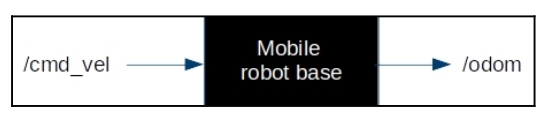
\includegraphics[scale=0.5]{vel_odom.png}
\caption{Inputs and outputs from the software point of view}
\end{figure}

\subsection{ROS messages format}

\verb|/cmd-vel| is of the \verb|geometry_msgs/Twist| message format. The message structure can be found in the following \href{http://docs.ros.org/melodic/api/geometry_msgs/html/msg/Twist.html}{link}
%
\verb|/odom| is of the \verb|nav_msgs/Odometry| message format. The message structure can be found in the following \href{http://docs.ros.org/melodic/api/nav_msgs/html/msg/Odometry.html.}{link}
%
Not all the fields are necessary in the case of our robot base since our robot is a 2 degrees of freedom robot.

\subsection{ROS controllers}

We would define the robot base's differential kinematics model using the \verb|diff_drive_controller| plugin. This plugin defines the robot equation we saw earlier. It helps our robot to move in space. More information about this controller is available at the \href{http://wiki.ros.org/diff_drive_controller} {website}.

\subsection{Modeling the robot base}

Now that we have all the necessary information about the robot, let's get straight into modeling the robot. The robot model we are going to build is as follows:

\begin{figure}
\centering
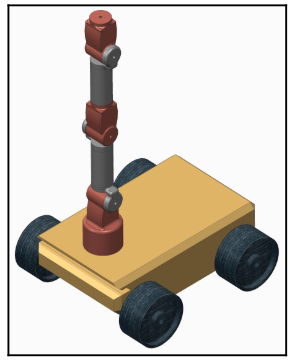
\includegraphics[scale=0.5]{render_robot.png}
\caption{Mobile manipulator to control.}
\end{figure}

There is something you need to know before you come out with thoughts about modeling robots using URDF. You could make use of the geometric tags that define standard shapes such as cylinder, sphere, and boxes, but you cannot model complicated geometries or style them. These can be done using third-party software, for example, sophisticated Computer Aided Design (CAD) software such as Creo or Solidworks or using open source modelers such as Blender, FreeCAD, or Meshlab. Once they are modeled, they're are imported as meshes. The models in this book are modeled by such open source modelers and imported into URDFs as meshes. Also, writing a lot of XML tags sometimes becomes cumbersome and we might get lost while building intricate robots. Hence, we shall make use of macros in URDF called xacro (\verb|http://wiki.ros.org/xacro|), which will help to reduce our lines of code for simplification and to avoid the repetition of tags.

Our robot base model will need the following tags:
\begin{itemize}
\item \verb|<xacro>|: To help define macros for reuse.
\item \verb|<links>|: To contain the geometric representations of the robot and visual information.
\item \verb|<inertial>|: To contain the mass and moment of inertia of the links.
\item \verb|<joints>|: To contain connections between the links with constraint definitions <Gazebo>: To contain plugins to establish a connection between Gazebo and ROS, along with simulation properties.

\end{itemize}

\begin{figure}
\centering
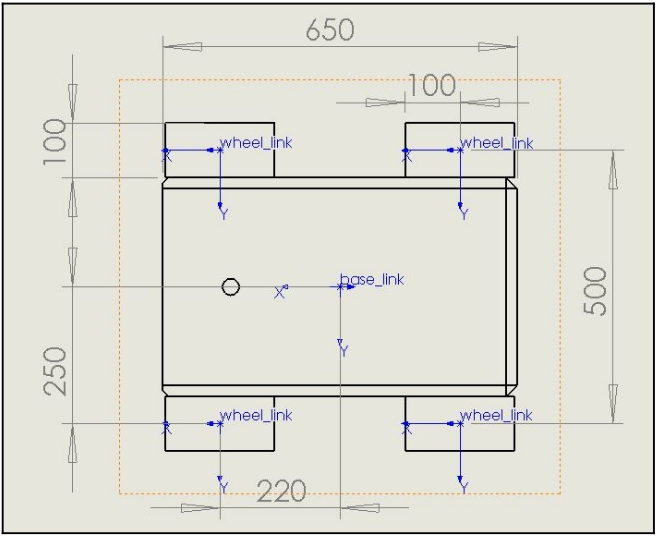
\includegraphics[scale=0.5]{mobile_measurements.png}
\caption{General measurement of the mobile base.}
\end{figure}

The chassis is named \verb|base_link| and you can see the coordinate system in its center. Wheels (or \verb|wheel_frames|) are placed with respect to the \verb|base_link| frame. You can see that, as per our REP, the model follows the right-hand rule in the coordinate system. You can now make out that the forward direction of the robot will always be toward the x axis and that the rotation of the robot is around the z axis. Also, note that the wheels rotate around the y axis with respect to its frame of reference (you shall see this reference in the code in the next section).

\subsection{Initializing Workspace}

All we need to do now is define those meshes as \verb|<link>| and \verb|<joint>| tags for our robot. The mesh files are available in this \href{https://github.com/nikorose87/robotics_labs/tree/main/Lab2/Resources/meshes}{link}. Follow these steps to initialize the workspace:

\begin{enumerate}
\item Let's create an ROS package and add our files to it. Create a package using the following commands in a new Terminal: 
\lstinputlisting[language=bash]{create_pkg.sh}
\item Create folders inside:
\begin{lstlisting}
mkdir config launch meshes urdf
\end{lstlisting}
\item Copy the meshes that you downloaded from the previous link and paste them into the meshes folder. Now, go to the urdf folder and create a file called \verb|robot_base.urdf.xacro| using the following commands:

\begin{lstlisting}
cd ~/chapter3_ws/src/robot_description/urdf/
gedit robot_base.urdf.xacro
\end{lstlisting}
\item Initialize the XML version tag and \verb|<robot>| tag, as shown here, and begin copying the given XML code into it step by step:
\begin{lstlisting}
<?xml version="1.0"?>
<<robot xmlns:xacro="http://ros.org/wiki/xacro" name="robot_base">
    
</robot>
\end{lstlisting}

\end{enumerate}

\subsection{Defining the links}

Since you're defining the robot model by parts, copy all of the following code here into the \verb|<robot>| tags (that is, the space between the \verb|<robot>| tags). The chassis link is as follows:

\lstinputlisting[language=xml]{base_link.xml}

The link defines the robot geometrically and helps in visualization. The preceding is the robot chassis, which we will call \verb|base_link|.

Four wheels need to connect to \verb|base_link|. We could reuse the same model with different names and necessary coordinate information with the help of xacro. So, let's create another file called \verb|robot_essentials.xacro| and define standard macros so that we can reuse them:

\begin{lstlisting}[language=xml]
<?xml version="1.0"?>

<robot xmlns:xacro="http://ros.org/wiki/xacro" name="robot_essentials" >

<xacro:macro name="robot_wheel" params="prefix">

<link name="${prefix}_wheel">
    <inertial>
      <origin
        xyz="-4.1867E-18 0.0068085 -1.65658661799998E-18"
        rpy="0 0 0" />
      <mass
        value="2.6578" />
    <visual>
      <origin
        xyz="0 0 0"
        rpy="1.5707963267949 0 0" />
      <geometry>
        <mesh filename="package://robot_description/meshes/wheel.stl" />
      </geometry>
      <material
        name="">
        <color
          rgba="0.79216 0.81961 0.93333 1" />
      </material>
    </visual>
  </link>

</xacro:macro>
</robot>
\end{lstlisting}

We have created a common macro for a wheel in this file. So, all you need to do now is call this macro in your actual robot file, \verb|robot_base.urdf.xacro|, as shown here:

\begin{lstlisting}[language=xml]
<xacro:robot_wheel prefix="front_left"/>
<xacro:robot_wheel prefix="front_right"/>
<xacro:robot_wheel prefix="rear_left"/>
<xacro:robot_wheel prefix="rear_right"/>
\end{lstlisting}

That's it. Can you see how quickly you have converted that many lines of code (for a link) into just one line of code for each link? Now, let's learn how to define joints.

\subsection{Defining the joints}

As shown in the preceding representation diagram, the connections are only between the wheels and the chassis. The wheels are connected to \verb|base_link| and they rotate around their y axis on their own frame of reference. Due to this, we can make use of continuous joint types. Since they're the same for all wheels, let's define them as xacro in the \verb|robot_essentials.xacro| file:

\begin{lstlisting}[language=xml]
<xacro:macro name="wheel_joint" params="prefix origin">

<joint name="${prefix}_wheel_joint" type="continuous">
    <axis xyz="0 1 0"/>
    <parent link ="base_link"/>
    <child link ="${prefix}_wheel"/>
    <origin rpy ="0 0 0" xyz= "${origin}"/>
  </joint>

</xacro:macro>
\end{lstlisting}

As you can see, only the origin and the name needs to change in the preceding block of code. Hence, in our \verb|robot_base.urdf.xacro| file, we'll define the wheel joints as follows:

\begin{lstlisting}[language=xml]
<xacro:wheel_joint prefix="front_left" origin="0.220 0.250 0"/>
<xacro:wheel_joint prefix="front_right" origin="0.220 -0.250 0"/>
<xacro:wheel_joint prefix="rear_left" origin="-0.220 0.250 0"/>
<xacro:wheel_joint prefix="rear_right" origin="-0.220 -0.250 0"/>
\end{lstlisting}

Now that you have everything in your file, let's visualize this in rviz and see whether it matches our representation. You can do that by using the following commands in a new Terminal:

\begin{lstlisting}[language=bash]
source /opt/ros/noetic/setup.bash
cd ~/chapter3_ws/ 
source devel/setup.bash 
roscd robot_description/urdf/
roslaunch urdf_tutorial display.launch model:=robot_base.urdf.xacro
\end{lstlisting}

Add the robot model and, in the \textbf{Global} options, set \textbf{Fixed Frame} to \verb|base_link|. Now, you should see our robot model if everything was successful. You can add the tf display and see whether the representation matches the \textit{Representing the robot 2D with link/coordinate system information diagram}. You can also move the wheels using the sliders that were launched as a result of setting the \verb|gui| argument to \verb|true|.

\section{Simulating the robot base}

The first four steps were initially used to define the robot URDF model so that it could be understood by ROS. Now that we have a proper robot model that is understood by ROS, we need to add a few more tags to view the model in Gazebo.

\subsection{Defining Collisions}

To visualize the robot in Gazebo, we need to add the <collision> tags, along with the <visual> tags defined in the <link> tag. For the base, add them to the \verb|robot_base.urdf.xacro| file since we defined \verb|base_link| there.

\begin{lstlisting}[language=xml]
    <collision>
      <origin
        xyz="0 0 0"
        rpy="1.5707963267949 0 3.14" />
      <geometry>
        <mesh filename="package://robot_description/meshes/robot_base.stl" />
      </geometry>
    </collision>
\end{lstlisting}

For all the wheel links, add them to the \verb1robot_essentials.xacro1 file since we defined the wheel link there:

\begin{lstlisting}[language=xml]
    <collision>
      <origin
        xyz="0 0 0"
        rpy="1.5707963267949 0 0" />
      <geometry>
        <mesh filename="package://robot_description/meshes/wheel.stl" />
      </geometry>
    </collision>
\end{lstlisting}

Since Gazebo is a physics simulator, we define the physical properties using the \verb|<inertial>| tags. We can acquire the mass and inertial properties from this third-party software. The inertial properties that are acquired from this software are added inside the \verb|<link>| tag, along with suitable tags, as indicated:

\begin{enumerate}
\item For the base:

\begin{lstlisting}[language=xml]
    <inertial>
      <origin
        xyz="0.0030946 4.78250032638821E-11 0.053305"
        rpy="0 0 0" />
      <mass
        value="47.873" />
      <inertia
        ixx="0.774276574699151"
        ixy="-1.03781944357671E-10"
        ixz="0.00763014265820928"
        iyy="1.64933255189991"
        iyz="1.09578155845563E-12"
        izz="2.1239326987473" />
    </inertial>
\end{lstlisting}

\item For the wheels:

\begin{lstlisting}[language=xml]
    <inertial>
      <origin
        xyz="-4.1867E-18 0.0068085 -1.65658661799998E-18"
        rpy="0 0 0" />
      <mass
        value="2.6578" />
      <inertia
        ixx="0.00856502765719703"
        ixy="1.5074118157338E-19"
        ixz="-4.78150098725052E-19"
        iyy="0.013670640432096"
        iyz="-2.68136447099727E-19"
        izz="0.00856502765719703" />
    </inertial>
\end{lstlisting}

\end{enumerate}

Now that the Gazebo properties have been created, let's create the mechanisms.

\subsection{Defining actuators}

Now, we need to define the actuator information for our robot wheels in the \verb|robot_base_essentials.xacro| file:

\begin{lstlisting}[language=xml]
<xacro:macro name="base_transmission" params="prefix ">

<transmission name="${prefix}_wheel_trans" type="SimpleTransmission">
  <type>transmission_interface/SimpleTransmission</type>
  <actuator name="${prefix}_wheel_motor">
   <hardwareInterface>hardware_interface/VelocityJointInterface</hardwareInterface>
   <mechanicalReduction>1</mechanicalReduction>
  </actuator>
  <joint name="${prefix}_wheel_joint">
   <hardwareInterface>hardware_interface/VelocityJointInterface</hardwareInterface>
  </joint>
</transmission>

</xacro:macro>
\end{lstlisting}

Let's call them in our robot file as macros:

\begin{lstlisting}[language=xml]
<xacro:base_transmission prefix="front_left"/>
<xacro:base_transmission prefix="front_right"/>
<xacro:base_transmission prefix="rear_left"/>
<xacro:base_transmission prefix="rear_right"/>
\end{lstlisting}

You can find the \verb|robot_base_essentials.xacro| file in this GitHub \href{https://github.com/nikorose87/robotics_labs/tree/main/Lab2/Resources/urdf}{repository}.

Now that the mechanisms have been called, let's call the controllers that use them and make our robot dynamic.

\section{Defining ROS CONTROLLERS}

Finally, we need to port the plugins that are needed to establish communication between Gazebo and ROS. For these, we need to create another file called \verb|gazebo_essentials_base.xacro| that will contain the \verb|<Gazebo>| tags as follows:

\begin{lstlisting}[language=xml]
<?xml version="1.0"?>

<robot xmlns:xacro="http://ros.org/wiki/xacro" name="gazebo_essentials" >


<gazebo>
    <plugin name="gazebo_ros_control" filename="libgazebo_ros_control.so">
      <robotNamespace>/</robotNamespace>
      <controlPeriod>0.001</controlPeriod>
      <legacyModeNS>false</legacyModeNS>
    </plugin>
  </gazebo>
<!--################################ ROS-Controllers ######################################-->
<gazebo>
      <plugin name="diff_drive_controller" filename="libgazebo_ros_diff_drive.so">
        <legacyMode>false</legacyMode>
        <alwaysOn>true</alwaysOn>
        <updateRate>1000.0</updateRate>
        <leftJoint>front_left_wheel_joint, rear_left_wheel_joint</leftJoint>
        <rightJoint>front_right_wheel_joint, rear_right_wheel_joint</rightJoint>
        <wheelSeparation>0.5</wheelSeparation>
        <wheelDiameter>0.2</wheelDiameter>
        <wheelTorque>10</wheelTorque>
        <publishTf>1</publishTf>
        <odometryFrame>map</odometryFrame>
        <commandTopic>cmd_vel</commandTopic>
        <odometryTopic>odom</odometryTopic>
        <robotBaseFrame>base_link</robotBaseFrame>
        <wheelAcceleration>2.8</wheelAcceleration>
        <publishWheelJointState>true</publishWheelJointState>
        <publishWheelTF>false</publishWheelTF>
        <odometrySource>world</odometrySource>
        <rosDebugLevel>Debug</rosDebugLevel>
      </plugin>
</gazebo>

<xacro:macro name="wheel_friction" params="prefix ">

<gazebo reference="${prefix}_wheel">
 <mu1 value="1.0"/>
 <mu2 value="1.0"/>
 <kp value="10000000.0" />
 <kd value="1.0" />
 <fdir1 value="1 0 0"/>
</gazebo>

</xacro:macro>

</robot>
\end{lstlisting}

The call macro in the robot file is as follows:

\begin{lstlisting}[language=xml]

<xacro:wheel_friction prefix="front_left"/>
<xacro:wheel_friction prefix="front_right"/>
<xacro:wheel_friction prefix="rear_left"/>
<xacro:wheel_friction prefix="rear_right"/>

\end{lstlisting}

Now that we have defined the macros for our robot, along with the Gazebo plugins, let's add them to our robot file. This can be easily done by just adding the following two lines in the robot file inside the \verb|<robot>| macro tag:

\begin{lstlisting}[language=xml]
<xacro:include filename="$(find robot_description)/urdf/robot_base_essentials.xacro" />
<xacro:include filename="$(find robot_description)/urdf/gazebo_essentials_base.xacro" />
\end{lstlisting}

Now that the URDFs are complete, let's configure the controllers. Let's create the following config file to define the controllers we are using. For this, let's go to our workspace, go inside the config folder we created, and create a controller config file, as shown here:

\begin{lstlisting}[language=bash]

cd ~/chapter3_ws/src/robot_description/config/
gedit control.yaml

\end{lstlisting}

Now, copy the code that's available in this GitHub \href{https://github.com/nikorose87/robotics_labs/blob/main/Lab2/Resources/config/control.yaml}{repository}, into the file. Now that we have completed our \verb|robot_base| model, let's test it in Gazebo.

This laboratory is under construction, please continue with the guides from the book \citep{Gandhinathan2020}, I attached to this \href{https://github.com/nikorose87/robotics_labs/blob/main/Lab2/chapter3_remaining_part.pdf}{link}.


\section{Additional Work}

Replace the manipulator from this guide and add the manipulator you have already configured with the MoveIt assistant. Present the report with this manipulator, the movement is a bonus. Work in groups as always.

This project was taken from \cite{Gandhinathan2020}
\bibliographystyle{plain}
\bibliography{biblio.bib}
\end{document}